\documentclass[Report.tex]{subfiles}

\begin{document}

\begin{figure}
\center
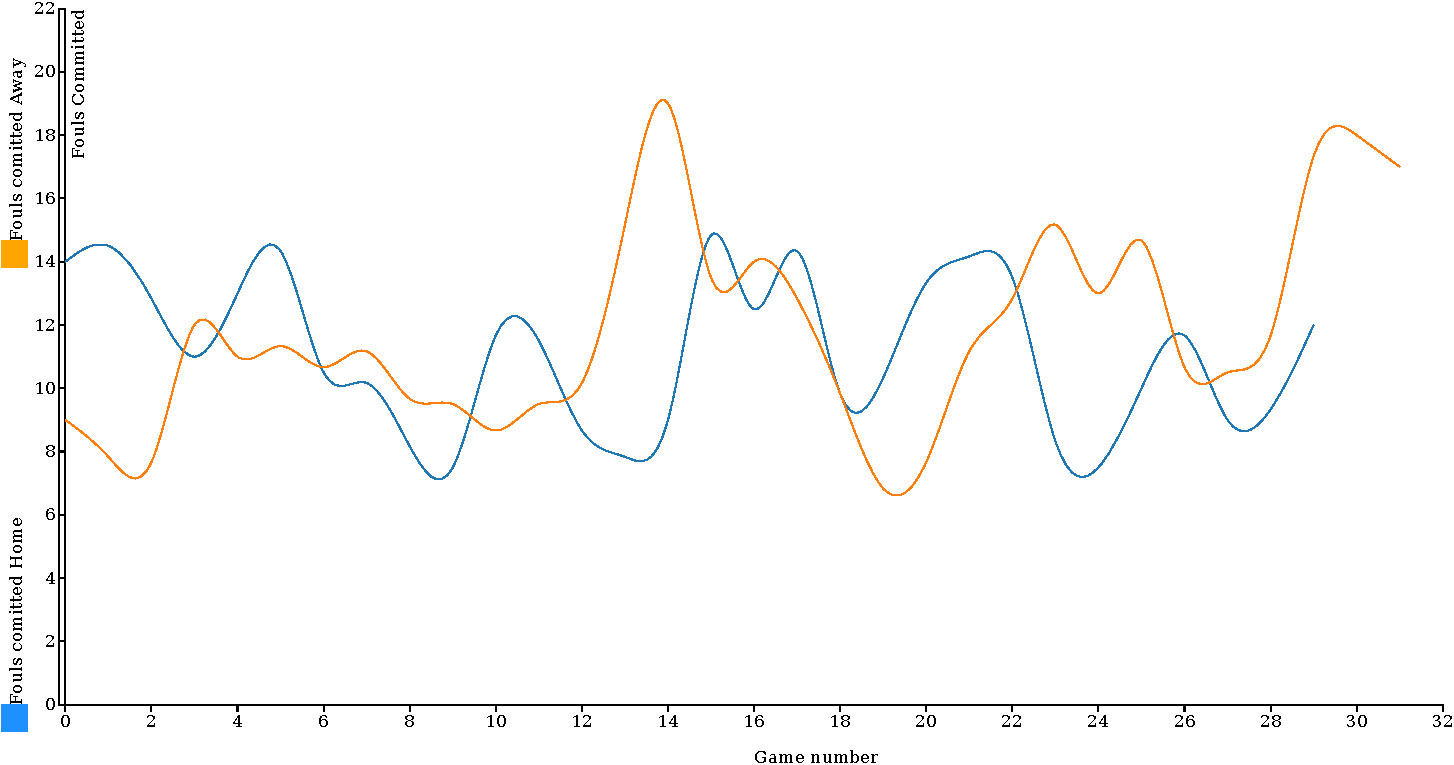
\includegraphics[width=\textwidth]{Figures/fouls.pdf}
\caption{A line chart showing fouls committed throughout a season, split up in those committed home, and those away.}
\label{Fig:FOULS}
\end{figure}


\paragraph{What-why-how\\\\}
Figure \ref{Fig:FOULS} shows fouls committed by SonderjyskE, throughout the season. It is split up in matches playing home, and away. On the x-axis we have the game number, showing how far into the season a game is, and on the y-axis, the number of fouls committed. In blue the number of fouls committed home and in orange the number committed away.\\

Attempting to confirm or invalidate the hypothesis of a team committing more fouls throughout the season, we chose to use a line chart, as it is an excellent way to give a quick overview, and quickly discover a trend in data if there is one. The matches was split up in home and away, due to the possibility that a team might be more comfortable playing at home than away, which could affect aggressiveness as well.\\

Gathering the data through the API, with the game-by-game statistics for a team, the information about fouls committed was extracted. This was done with a single loop, running through each event in the API response, resulting in complexity $O(n)$, where n is the number of events. Finally, the resulting data was processed in D3, to create the line chart shown in Figure \ref{Fig:FOULS}.

\paragraph{Findings\\}
As seen on Figure \ref{Fig:FOULS}, the fouls committed went up and down a lot, without any apparent trend. Even though there seem to be a spike in fouls committed toward the last few games, it is nothing more than the spikes seen earlier in the season. Worth noting is that the season is not finished at this point, which is why there are a few data points missing for the home matches.


\end{document}
